\chapter{Timeseries Analysis}


\section{Dataset Preparation}

To start our analysis we needed to once again prepare the dataset.
We started by working on the $final clean 3$ dataset by only keeping the incidents between 2014 and 2017 and by adding to each incident the week in which it took place.
Finally we created a dataframe called $clean city df$ in which we kept only the cities with a number of incidents greater than the 15$\%$ of incidents in the 209 weeks total.

\section{City Score}

For the first analysis on the motifs and anomalies we decided for a score that incorporated the number of killed people in each incident.
This score for each city is defines as follows:
\textit{Score $=$ number of killed people in that week + number of injured people in that week $* 0.8 +$ number of arrested people in that week $* 0.5 +$  number of child participants in that week $+$ number of teen participants in that week $* 0.8 +$ number of adult participants in that week $* 0.5$}
It can be considered as a positive weighted sum where the weights are chosen arbitrarily and can be changed based on the importance that we want to give to each indicator.
we gave a higher weight to the number of killed and injured people, and a lower weight to the number of arrested people
We also gave a higher weight to the number of children and teenagers involved in the incident, and a lower weight to the number of adults involved
Defined in this way the score can be interpreted as a measure of the severity of each incident.

\begin{figure}[ht]
    \centering
    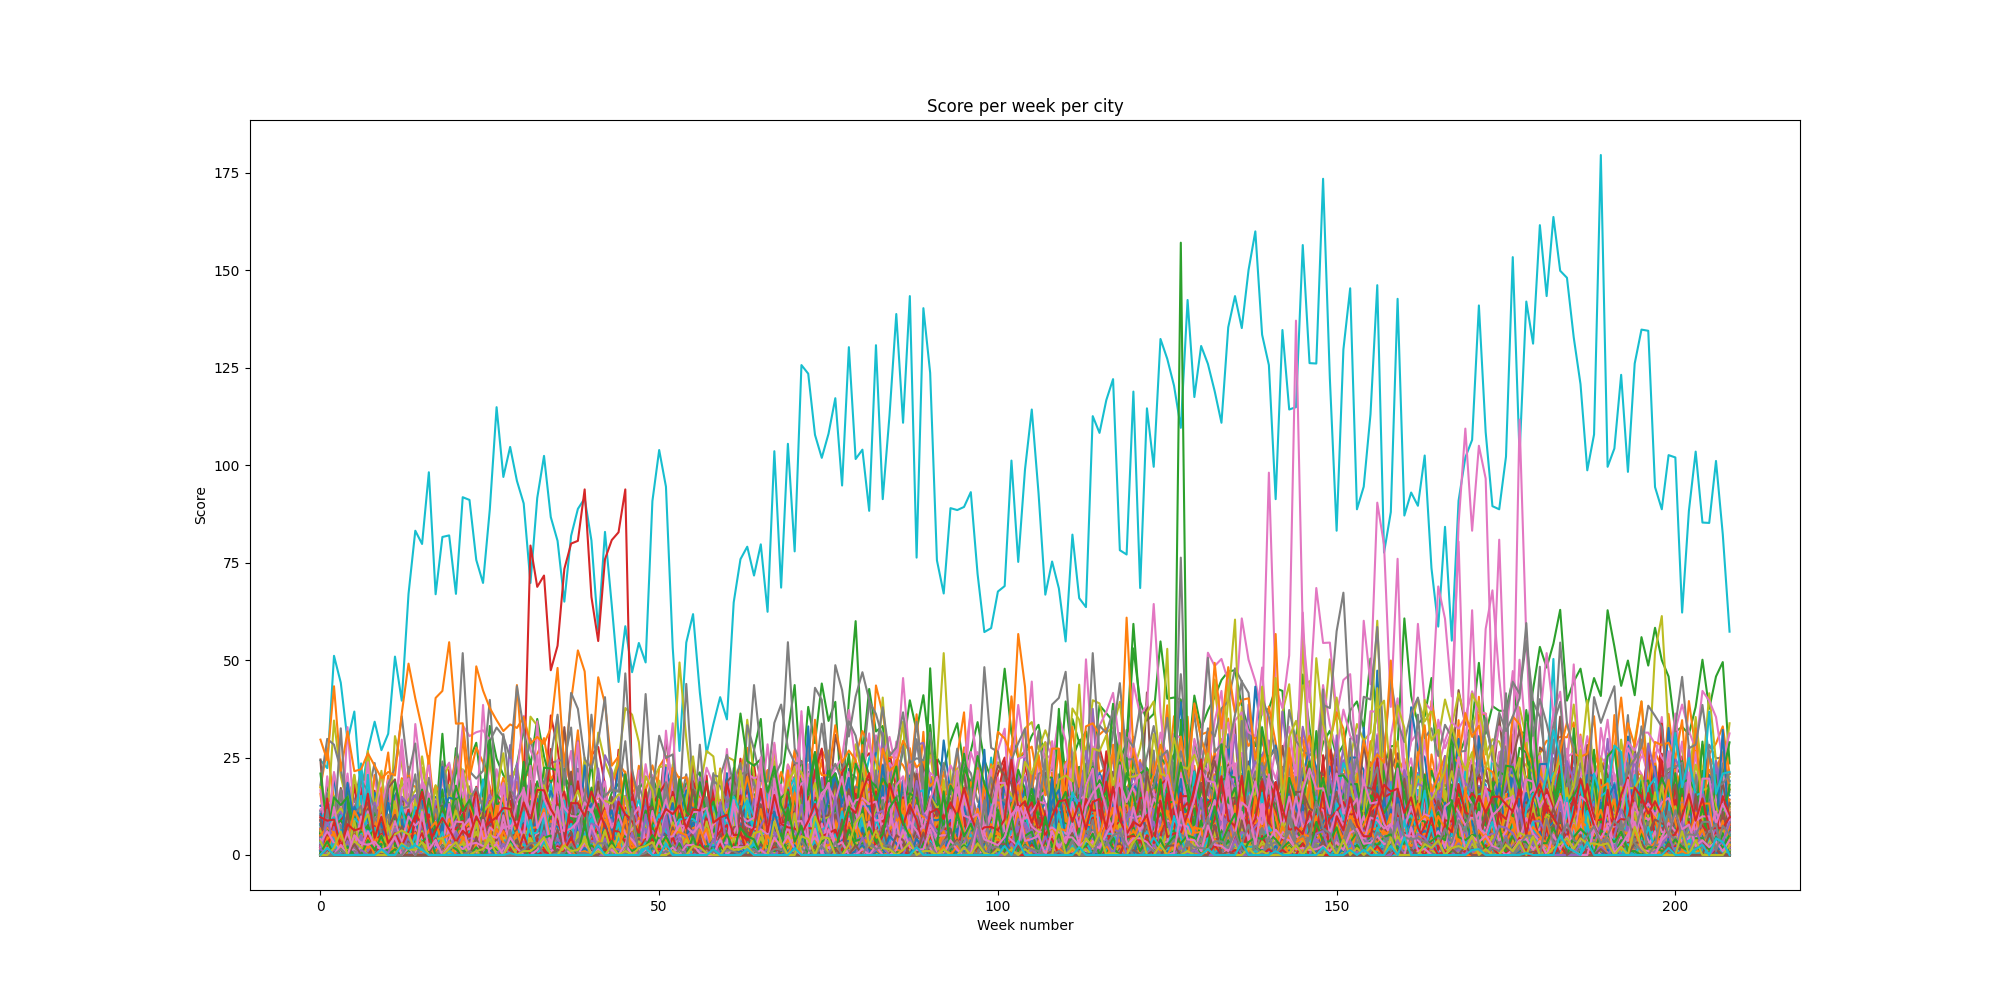
\includegraphics[width= 0.8\textwidth]{images/Capitolo1/score_per_week_per_city.png} 
    \caption{Questa è un'immagine} 
    \label{fig:score_per_week_per_city}
\end{figure}

\subsection{Scaled Timeseries}

We decided to also test the clustering on the timeseries scaled with the standard scaler and the minmax scaler, to see if doing so would result in better clusters

In the following figure we can see the plot for all the timeseries scaled in this way

\begin{figure}[ht]
    \centering
    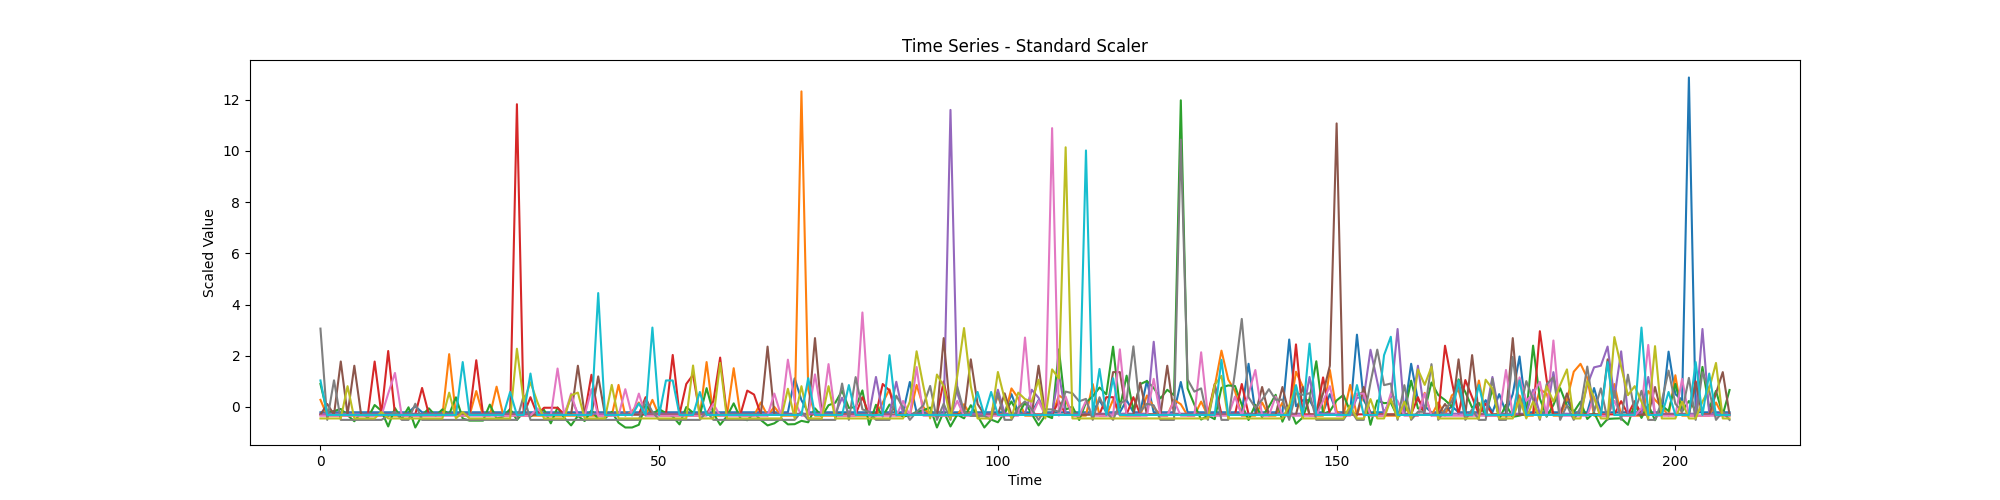
\includegraphics[width= 0.8\textwidth]{images/Capitolo1/time_series_standard_scaler.png} 
    \caption{Questa è un'immagine} 
    \label{fig:time_series_standard_scaler}
\end{figure}

\begin{figure}[ht]
    \centering
    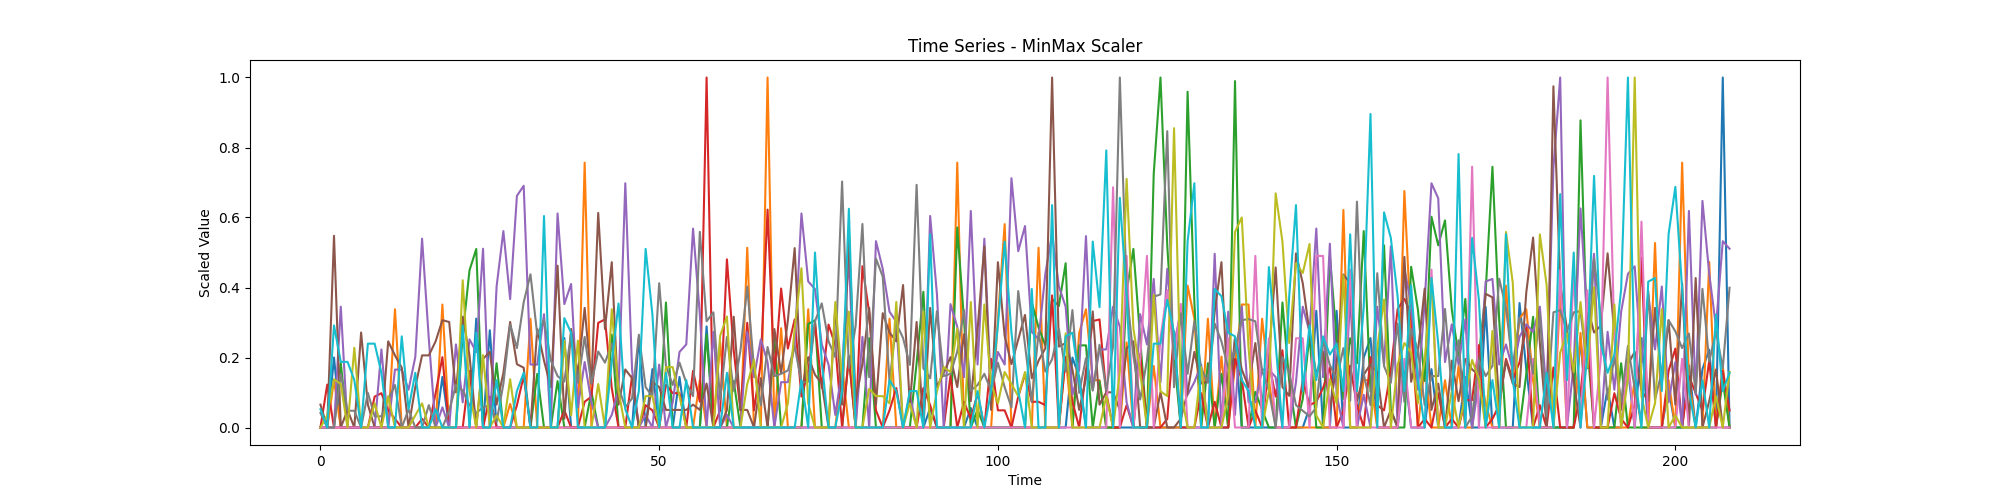
\includegraphics[width= 0.8\textwidth]{images/Capitolo1/time_series_minmax_scaler.png} 
    \caption{Questa è un'immagine} 
    \label{fig:time_series_minmax_scaler}
\end{figure}


\section{Clustering}

For the cluster analysis we decided to not test most of the algorithms because we already tested them in previous section of the project.
So we decided to concentrate on K-means on the raw time series and on their features.
We also skipped the euclidean distance and decided to use the Dynamic Time Warping (DTW) mainly because it is better suited to capture time series with varying pattern, time shifts or speed, all things that euclidean distance could miss.


\subsection{Clustering on the raw Timeseries}

We applied K-means on the original timeseries and also on the one scaled with the standard scaler and the minmax scaler.

To find the best number of cluster we used the same technique that we used in the clustering of the incident dataset, the silhouette score.

As seen in the table, both the standard scaler and the minmax scaler resulted in a significant reduction of the clustering score, while the original timeseries reached a 0.8. 


\subsection{Clustering on the feature of the Timeseries}

Another technique often used when dealing with Timeseries is to reduce each one of them to a vector containing some significant feature of the Timesearies, such as mean, variance, kurtosis ecc..  and then apply the clustering algorithms to those points.

Same as the clustering on raw time series we performed K-means on the initial timeseries, the timeseries scaled with the standard scaler and the one scaled with the minmax scaler.
We registered a significant increase in the silhouette score for all three of the timeseries, a number much greater than the one for the corresponding initial timeseries.
In particular feature clustering on the original timeseries seems to best differentiate the two clusters found





\subsection{Comparison of the clustering with a random walk}

To test how well K-means worked on our timeseries we generated the same number of random walk with the same number of points and with the same min and max value as our standard timeseries.

We then procedeed to use K-means on the standard random timeseries and discovered a silhouette score close to zero, confirming that our time series were clustered better than randomly.
The same conclusion was reached also on the feature based cluster, in which even though the clustering on the random timeseries reached $0.50$ it was still significantly lower than the corresponding score on the original timeseries




\section{Motif and Anomaly Detection}

The timeseries chosen for the motif discovery are the two cluster centroids found with K-means in the previous point.
Altough the significance of those two timeseries could be discussed, the idea behind it is that no timeseries is significant enough to conduct this kind of analysis on.
We should consider them equal and in this way analyze each city one by one.
Because it was not possible to study that many city, we opted to take the two timeseries that describe the two different clusters.
Another possible analysis could be conducted on a small sample from each of those clusters, but still this analysis is not that much more significant.

The only interesting thing that we can notice is the 'absence' of motifs in the random series, which is to be expected, while we can always find some motif in our timeseries, scaled or not scaled.

As far as Anomaly detection, we conducted it on the non scaled Timeseries, and we were able to find a couple of anomalies, but also these anomalies cannot really be interpreted in a nice way.

For comparison, we also took a couple of the cities with the highest score and the one with the lowest and conducte the motif and anomaly discovery on those.

The results were similar to the one on the cluster centers, because nothing particularly interesting emerged, except that the motif alternated between each other.



\section{Shapelets}

For the analysis on the Shapelets of the time series, we needed to create  new indicator.
The new score for each city is defined as follows:
\textit{Score\textunderscore Shapelet $=$ number of incidents in that week + number of participants in incidents in that week}

In this case the main idea behind this score is that by summing the number of incidents and the number of people involved we could get a decent indirect correlation with the given label is\textunderscore killed.

We chose the threshold after which a timeseries would be considered as a positive is\textunderscore killed value, in a way to make the number of positive city almost the same as the negative cities, mainly to make classification more precise.

For the shapelet extraction, due to the high computational cost of the algorithms, decided to take only a small sample of the time series and extract the shapelet from those.
We also tried to use the tensorflow library but gave results that suggested some kind of problem, so we used the alternative method for finding the shapelets (pyts library)

Despite the low number of samples, the F1 score of the classifier got an accuracy of 0.83 and a decent ROC curve




















